\documentclass[a4paper,norsk, 10pt]{article}
\usepackage[utf8]{inputenc}
\usepackage{verbatim}
\usepackage{listings}
\usepackage{graphicx}
\usepackage[norsk]{babel}
\usepackage{a4wide}
\usepackage{color}
\usepackage{amsmath}
\usepackage{float}
\usepackage{amssymb}
\usepackage[dvips]{epsfig}
\usepackage[toc,page]{appendix}
\usepackage[T1]{fontenc}
\usepackage{cite} % [2,3,4] --> [2--4]
\usepackage{shadow}
\usepackage{hyperref}
\usepackage{titling}
\usepackage{marvosym }
\usepackage{subcaption}
\usepackage[noabbrev]{cleveref}
\usepackage{cite}


\setlength{\droptitle}{-10em}   % This is your set screw

\setcounter{tocdepth}{2}

\lstset{language=c++}
\lstset{alsolanguage=[90]Fortran}
\lstset{alsolanguage=Python}
\lstset{basicstyle=\small}
\lstset{backgroundcolor=\color{white}}
\lstset{frame=single}
\lstset{stringstyle=\ttfamily}
\lstset{keywordstyle=\color{red}\bfseries}
\lstset{commentstyle=\itshape\color{blue}}
\lstset{showspaces=false}
\lstset{showstringspaces=false}
\lstset{showtabs=false}
\lstset{breaklines}
\title{FYS1120 Oblig 2}
\author{Daniel Heinesen}
\begin{document}
\maketitle

\paragraph*{Oppgave 2}
\subparagraph*{a)}
Med et uniformt magnetfelt vil kraften

\begin{equation}
\vec{F} = q \vec{v}\times \vec{B}
\end{equation}

alltid stå vikelrett på hastighetsvektoren, hvilket betyr at vi kan forvente en sikulærbane. Vi vil senere i oppgaven løse likningen for denne bevegelsen analytisk.\\

Programmet gir disse plottene:

\begin{figure}[H]
\begin{center}
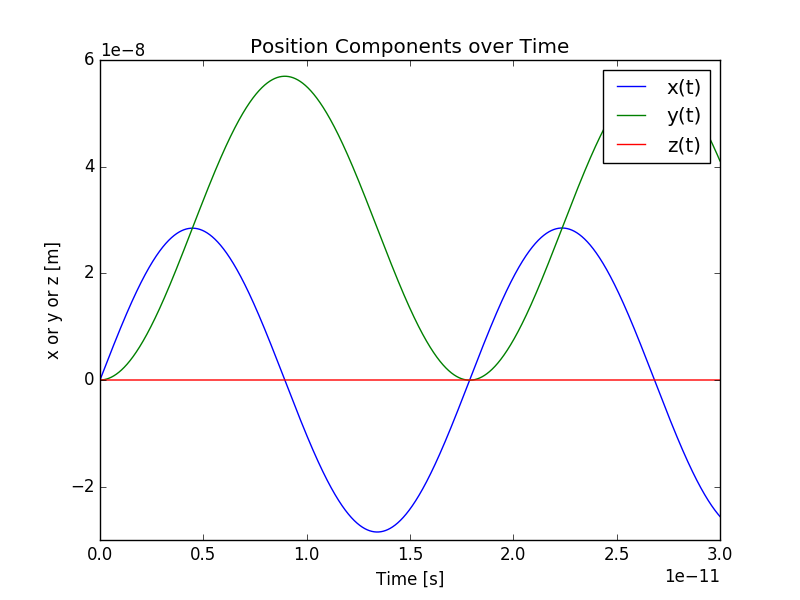
\includegraphics[width = 70mm]{opp2PosKomp2d.png}
\caption{$x$, $y$ og $z$ plottet mot tid.}
\end{center}
\end{figure}

Vi kan se at $x$ og $y$ varierer som en $cosinus$- og en $sinus$funksjon -- $x$ er noe forskyvet --, mens $z$ holder seg konstant på 0.

\begin{figure}[H]
\begin{center}
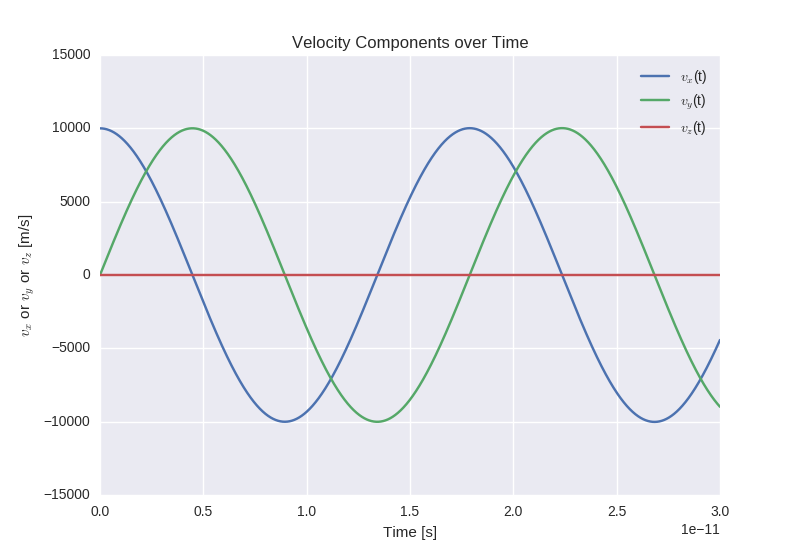
\includegraphics[width = 70mm]{opp2VelKomp2d.png}
\caption{$v_x$, $v_y$ og $v_z$ plottet mot tid.}
\end{center}
\end{figure}

Som med posisjonene er $z = 0$, og $x$ og $y$ varierer er $cosinus$- og en $sinus$funksjoner.

\begin{figure}[H]
\begin{center}
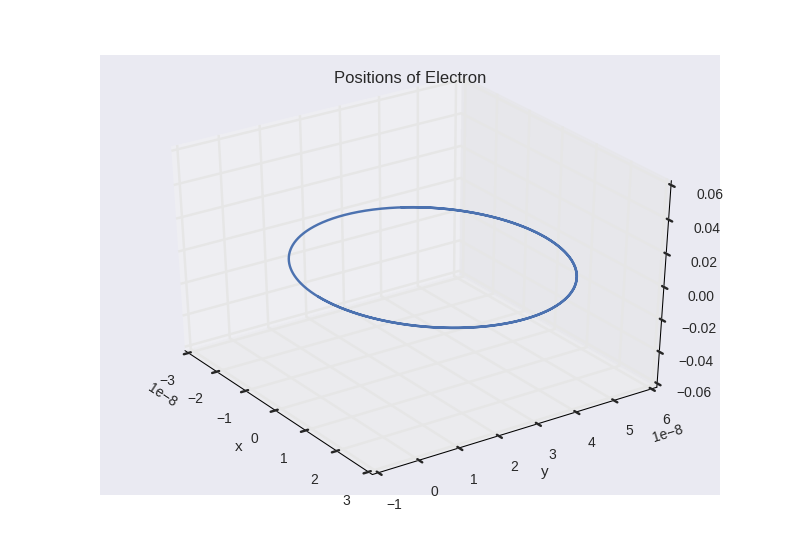
\includegraphics[width = 70mm]{opp2Pos3d.png}
\caption{Vi kan se at elektronet beveger seg i en sirkelbane, som vi forventet.}
\end{center}
\end{figure}

Vi kan se i figurene over at elektronet beveger seg i en sirkelbane, det var det vi forventet fra det lille resonnomentet i starten av oppgaven.

\subparagraph*{b)}
For å finne omløpstiden til numerisk kan vi bruke 2 metoder. Den visuelle og unøyaktige er å plotte $|\vec{r}|$ mot $t$:

\begin{figure}[H]
\begin{center}
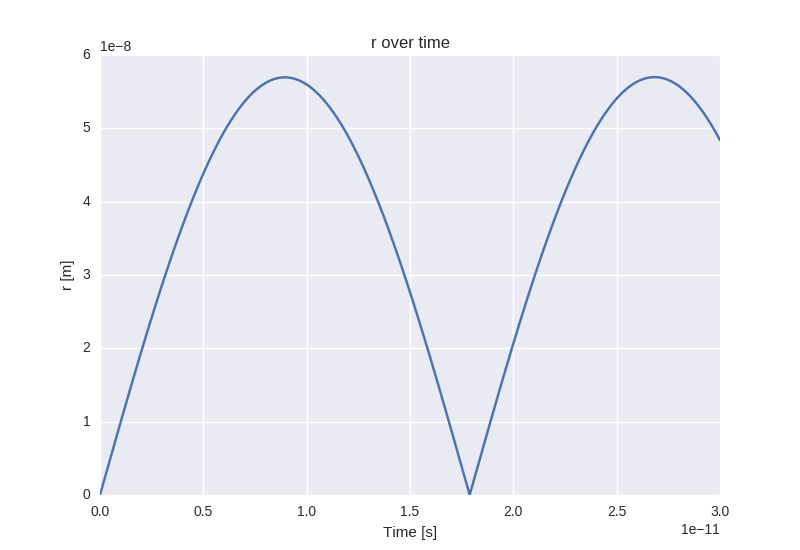
\includegraphics[width = 70mm]{opp2R2d.png}
\caption{Avstanden til origo over tid.}
\end{center}
\end{figure}

Vi kan finne omløpstiden ved å se når avstanden fra origo er 0. Vi kan se avstanden er 0 ca mellom $1.7$ og $1.8\cdot 10^{-11} $. En mer nøyaktig måte får å finne omløpstiden er å sjekke når vinkelen til elektronet i forhold til $x-aksen$. Omløpstiden vi får fra dette er $1.8021\cdot 10^{-11}$ s. Med det analytiske utrykket vi skal utlede om noen deloppgaver, finner vi en verdi på $1.789 \cdot 10^{-11} s$. Vi ser at det numeriske svaret er veldig likt det analytiske.

\newpage

\subparagraph*{c)}
For å finne syklotronfrekvesen ser vi at for å gå i en sirkerbane må størrelsen til kraften fra magnetfeltet være lik sentripitalkraften.

$$
F_{magnet} = F_{sentripital}
$$

\begin{equation}
qvB = m\frac{v^2}{r}
\end{equation}


\begin{equation}
R = \frac{vm}{qB}
\end{equation}

Vi bruker sammenhengen mellom frekvensen og radius:

\begin{equation}
\omega_s = \frac{v}{R} = \frac{vqB}{vm} = \frac{qB}{m}
\end{equation}


Perioden er tiden det tar å komme seg $2\pi$ rundt sirkelen med vinkelhastighet $\omega$

\begin{equation}
T = \frac{2\pi}{\omega} = \frac{2\pi m}{qB} = 1.789\cdot 10^{-11} s
\end{equation} 

\subparagraph*{d)}

Har elektronet en hastighet i z-retning, vil vi få en bane som skrur oppover.
Jeg bruker den analytiske løsningen, og plotten den over den numeriske. Den analytisk løsningen er gitt ved:

\begin{equation}
\begin{split}
r_x(t) = \frac{v_{x0}}{\omega}(1-\cos(\omega t))
\\
r_y(t) = -\frac{v_{x0}}{\omega}\sin(\omega t)
\end{split}
\end{equation}

For $x-$ og $y-retningen$ (Vises i Appendix A), og for $z-retning$

\begin{equation}
r_z(t) = v_{z}t
\end{equation}

Plottet blir da:

\begin{figure}[H]
\begin{center}
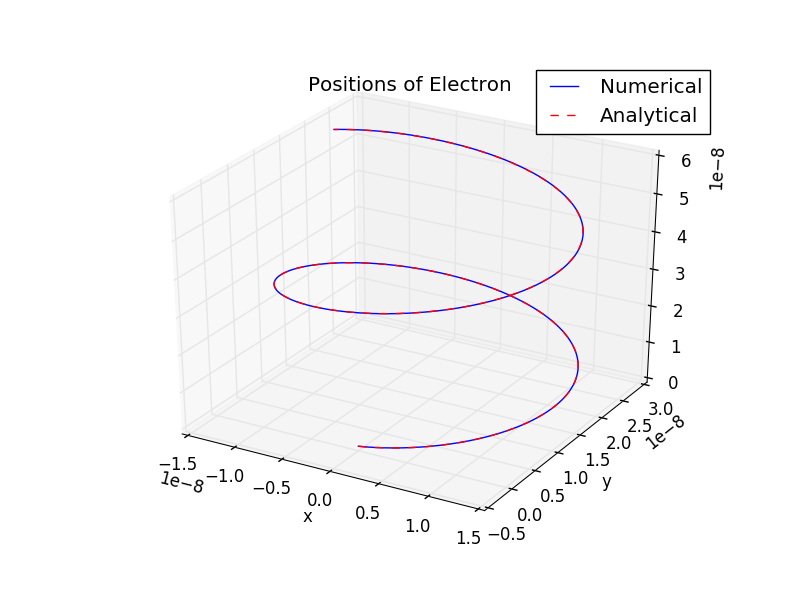
\includegraphics[width = 70mm]{opp2dPos3dwAnalytic.png}
\caption{Posisjonen til et elektron med en fart i $z-retning$.}
\end{center}
\end{figure}

En oppover skruebane. Vi kan se at den analytiske og numeriske løsningen er (mer eller mindre) helt like.

\newpage

\paragraph*{Oppgave 3}
\subparagraph*{a)}
I mitt program bruker jeg et magnet felt på $B = 2T$. Jeg får da:

\begin{figure}[H]
\begin{center}
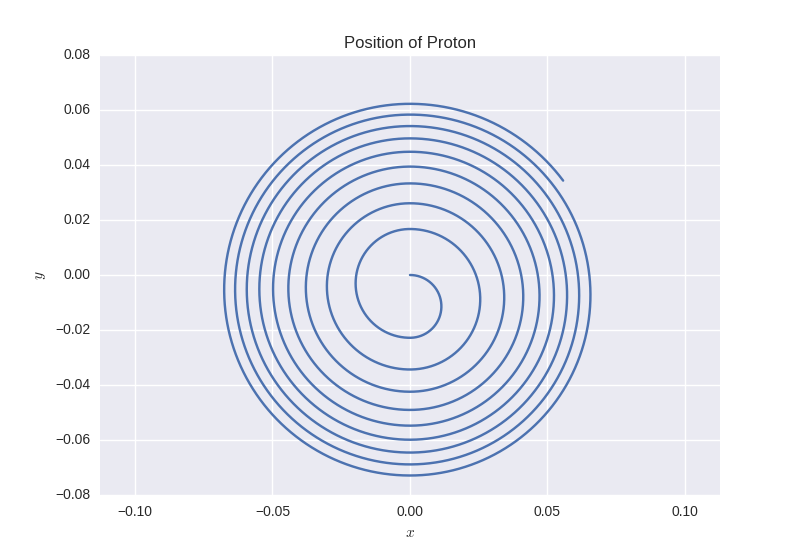
\includegraphics[width = 70mm]{opp3aPos.png}
\caption{En sirkelbane med økende radius.}
\end{center}
\end{figure}

Protonet akselereres når det går gjennom det elektriske feltet i $the valley gap$, og bøyes i det magnetiske feltet. E-feltet varierer slik at protonen alltid akselereres i hastighetsretningen. Dette resulterer i en sirkelbevegelse hvor radiusen øker for hver gang protonet går gjennom $valley gapet$\\

For hver gang protonet passerer det elektriske felten vil det akselerere. Den totale hastighetsforandringen protonet har fått i E-feltet er avhengig av hvor lang tid det var i feltet. Jo større radiusen på sirkelbanene er, jo høyerer er farten. Dette betyr at ved større radiuser bruker protonet ikke like lang tid i E-feltet som ved mindre radiuser. Det får derfor ikke like stor hastighetsforandre, hvilket resulterer med at radien på den neste omdreiningen ikke øker like mye. Oppsummert i én setning blir økningen til radiusen mindre for hver omdreining fordi hastigheten blir større og protonen tilbringer mindre tid i E-feltet og får mindre akslerasjon hver omdreining.

\subparagraph*{b)}

Vi lar nå protonet slippes løs fra syklotronen når avstanden fra sentrum er $90 \mu m$ får vi:

\begin{figure}[H]
\begin{center}
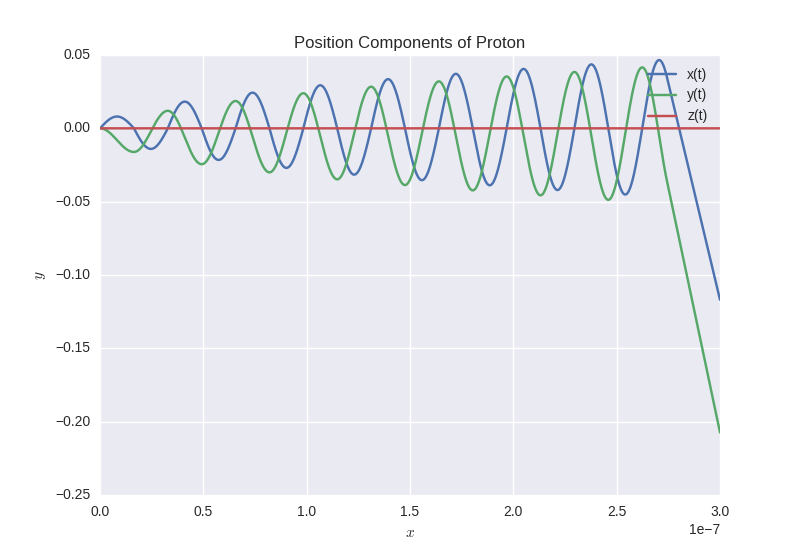
\includegraphics[width = 70mm]{opp3bPosKomp.png}
\caption{Plott av $x$, $y$ og $z$ over tid.}
\end{center}
\end{figure}

Som i oppgave 2 får vi $cosinus-$ og $sinusfunksjoner$ for $x$ og $y$, og en konstant $z$. Siden radiusen øker vil amplitudene $cosinus-$ og $sinusfunksjonen$ øke. Etter $90 \mu m$ slipper protonet løs og fortsetter i den retningen den hadde.

\begin{figure}[H]
\begin{center}
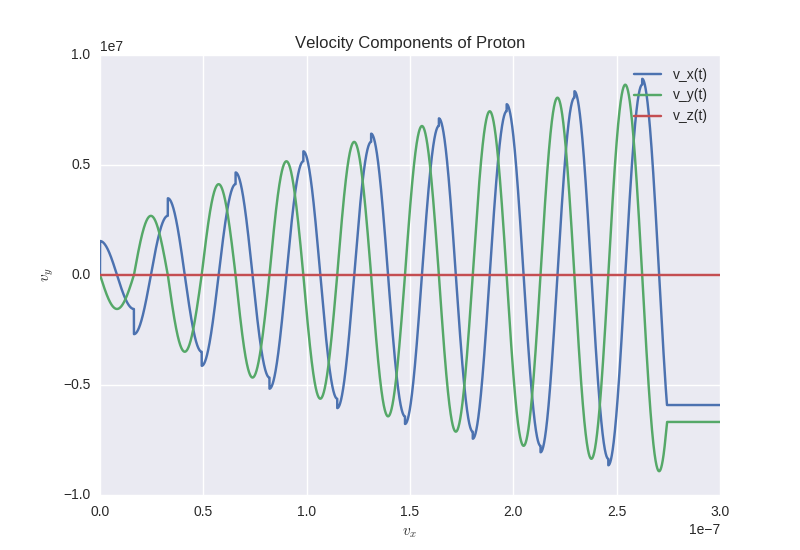
\includegraphics[width = 70mm]{opp3bVelKomp.png}
\caption{Plott av $v_x$, $v_y$ og $v_z$ over tid.}
\end{center}
\end{figure}

$v_x$, $v_y$ og $v_z$ likner mye på posisjonskomponentene. Vi kan se at $v_x$ plutselig øker nær topp- og bunnpunktene. Dette er når protonet akelsereres i E-feltet. På slutten slippes protonet løs og protonet opplever ingen akselerasjon og hastigheten forblir konstant.


\subparagraph*{c)}

Her er et plot av farten over tid:

\begin{figure}[H]
\begin{center}
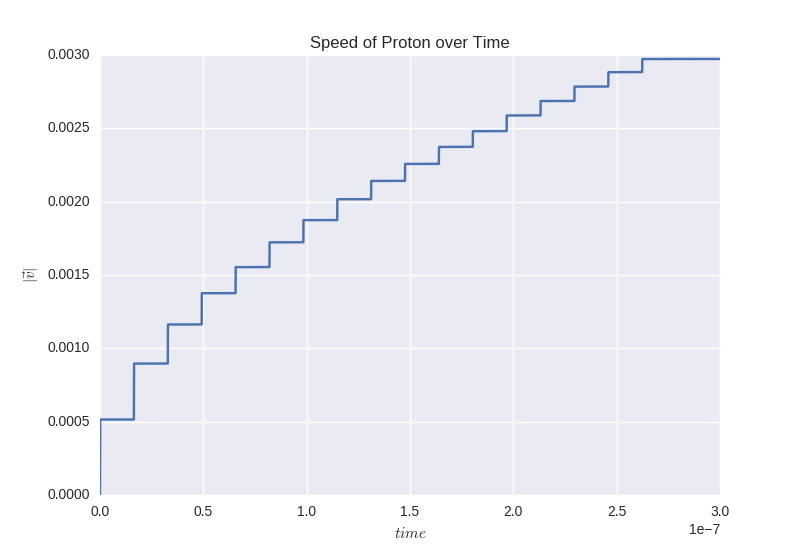
\includegraphics[width = 70mm]{opp3bSpeed.png}
\caption{Farten til protonet som en faktor av lyshastigheten $c$.}
\end{center}
\end{figure}

Vi kan se farten øker brått når protonet går gjennom E-feltet, for så å bli konstant når det bare påvirkes av magnetfeltet. Vi kan se at mot sluttet blir farten konstant. Tar vi å sjekker lengden av hastighetsvektoren i siste tidspunkt finner vi unnslipsfarten:

$$
|\vec{v}_{last}| = 8918994.96 m/s = 0.00297 c
$$

\subparagraph*{d)}

Vi bruker $|\vec{F}| = qvB$ og løser uttrykket for v, og får:
\begin{equation}
v = \frac{qBr}{m} 
\end{equation}

Vi setter nå dette uttrykke som hastigheten i den kinetiske energien:

\begin{equation}
E = \frac{1}{2}mv^2 = \frac{1}{2} \frac{q^2B^2r^2}{m}
\end{equation}


\subparagraph*{e)}

Jeg fant en artikkel kalt "Modern compact accelerators of cyclotron type for medical applications"  \cite{Smirnov2016}. I artikkelen var det oppgitt parameterene for mange syklotroner. Jeg valge den første syklatronen i artikkelen og brukte dens parametere til å regne ut energien, og sammenliknet den med energien de ga i artikkelen:\\

\begin{center}
\begin{tabular}{|c|c|c|c|}
\hline
$r_D$ & $B$ & $E_{gitt}$ & $E_{utregnet} $ \\ \hline
$115 mm$  & $4.5 T$ & $12.5 MeV$ & $12.81 MeV$ \\ \hline
\end{tabular}
\end{center}

Vi kan se at den oppgitte og min utregnede energi stemmer veldig godt over ens. Dette har med at den syklatronen jeg valgte var den minste i artikkelen. Siden den var så liten, vil ikke protonet få en så stor hastighet at relativitet begynner å spille en rolle.


\paragraph*{Oppgave 4}

\subparagraph*{a)}

Gauss lov:

$$ \Phi_E = \oint \textbf{E} \times d \textbf{A} = \dfrac{Q}{\epsilon_0}$$

\textbf{Oppgave 4a}


E-feltet vi skal regne ut her har 2 deler, en som er inne i kulen $r < R$ og utenfor kulen $r >= R$. Vi starter med feltet inne i kulen:\\

 
Siden ikke all ladningen er med innfører vi en ladningstetthet $\lambda = \frac{Q_{tot}}{V_{kule}}$. Vi kan bruke det til å finne ladningen i en radius $r$: 
$$ q = \lambda \dfrac{4}{3} \pi r^{3} $$

Siden gauss-flaten alltid står normalt på E-feltet, vil kryss produktet blir redusert til $\bold{E} \times d\bold{A} = EdA$. Fra Gauss lov får vi da:

$$ \Phi = EA = E 4 \pi r^2 = \dfrac{q}{\epsilon_0} $$

$$ \Rightarrow E\cdot 4 \pi r^2 =  \dfrac{4\lambda  \pi r^3}{3\epsilon_0} $$

$$ E = \frac{\lambda r}{3\epsilon_0} $$

Setter inn $\lambda = \frac{3Q}{4\pi R^3}$

\begin{equation}
E(r) = \dfrac{1}{4 \pi \epsilon_0} \cdot \dfrac{Qr}{R^3}
\end{equation}



\subparagraph*{b)}

På en flate (liggende langs x-aksen for å gjøre det enkelt å forklare under) vil en tilfeldig punkt midt i flaten bare ha et E-felt som peker rett opp i y-retning. Dette er fordi dens E-felt i x-retning vil bli kansellert av nabopunktene som som har en like stort med motsatt rettet felt i x-aksen. Rett oppover på y-aksen vil feltet til alle punkene peke sammeretning, og vil ikke bli kansellert. Nær endene vil punktene ikke ha like mange naboer, og det vil dannes et felt i x-retning også. Siden vi har en uendelig stor flate, vil vi ikke ha noen kanter, og vi vil ikke få randeffekten. Dette betyr at E-feltet peker rett opp over alt. Vi kan derfor lage en gaussflate formet som en boks hvor som helst på flaten. \\ 

Siden vi dekker en liten del av flaten med en boks, må vi bruke ladningstettheten $\sigma$. Ladningen inne i flaten blir da $q = \sigma s^2$, der $s$ er lengden på sidene på boksen. For den delen av boksen som er parallelt med feltet, vil fluksen være 0 (pga kryssproduktet), så fluksen avhenger bare av toppen og bunnen på boksen med areal $A=s^2$

$$
\Phi = EA = E \cdot 2s^2  = \dfrac{q}{\epsilon_0} = \dfrac{\sigma s^2}{\epsilon_0}
$$

\begin{equation}
E(r) = \frac{\sigma}{2\epsilon_0}
\end{equation}

Med andre ord er styrken på E-feltet uavhengig av avstanden fra flaten.


\subparagraph*{c)}

Vi har nå en uendelig lang stav (liggende på y-aksen). Av samme grunn som på flaten, vil det nå ikke gå et E-felt langs y-aksen. Vi kan derfor legge en gaussflaten formet som sylinder rundt staven. Fluksen langs bunnen og toppen på sylinderen vil være 0 siden de ligger parallelt på feltet. Vi bruker at ladingen inne i gaussflaten er $q = \lambda L$, hvor $L$ er høyden på sylinderen.



$$ \Phi = EA = E \cdot 2 \pi r L = \frac{q}{\epsilon_0} \dfrac{\lambda L}{\epsilon_0} $$

Vi får da:

\begin{equation}
E(r) = \frac{1}{2\pi \epsilon_0}\cdot \frac{\lambda}{r}
\end{equation}

\bibliography{ref} 
\bibliographystyle{plain}

\newpage

\paragraph*{Kode:}
\hspace{5mm}

\lstinputlisting{oppgave3b.py}

\newpage


\paragraph*{Appedix A: Utreging av analytisk løsning.}
\hspace{5mm}

Vi skal vise at vi får en sirkelbane i oppgave 2, ved å løse problemet analytisk:\\

Vi starter med at

\begin{equation}
\vec{a} = \frac{q}{m}(\vec{v} \times \vec{B})
\end{equation}

Vi setter det så opp komponentvis, siden vi bare har et magnetfelt i z-retning, setter vi $B_z = B$:

$$
\vec{v} \times \vec{B} = \hat{i}(v_yB) - \hat{j}(v_xB)
$$

\begin{equation}
\begin{split}
a_x = v_x' = - \frac{qB}{m}v_y
\\
a_y = v_y' =  \frac{qB}{m}v_x
\end{split}
\end{equation}

vi bruker at $\frac{qB}{m} = \omega$(vises i en senere deloppgave). Den generelle løsningen på denne differensiallikningen er:

\begin{equation}
\begin{split}
v_x(t) = c_1\sin(\omega t) + c_2\cos(\omega t)
\\
v_y(t) = c_1\cos(\omega t) - c_2\sin(\omega t)
\end{split}
\end{equation}

setter vi inn grensebetingelsene $v_x(0) = v_{x0}$ og $v_y(0) = 0$ får vi 

\begin{equation}
\begin{split}
v_x(t) = v_{x0}\cos(\omega t)
\\
v_y(t) = -v_{x0}\sin(\omega t)
\end{split}
\end{equation}

Om vi integrerer dette og setter inn at $r_x(0) = r_y(0) = 0$ får vi et uttrykk for posisjonen:

\begin{equation}
\begin{split}
r_x(t) = \frac{v_{x0}}{\omega}(1-\cos(\omega t))
\\
r_y(t) = -\frac{v_{x0}}{\omega}\sin(\omega t)
\end{split}
\end{equation}

Dette gir oss en sirkelbevegelse hvor x-komponenten er litt forskyvet, akkurat som vi så i den første figuren. Radiusen på sirkelen er $R = \frac{v_{x0}}{\omega}$. 





\end{document}


